\documentclass[twocolumn,twoside,11pt]{article}

\usepackage[portuguese]{babel}  % portuguese
\usepackage{graphicx}           % images: .png or .pdf w/ pdflatex; .eps w/ latex

\usepackage{lipsum}             % generate dummy text throughout this template

%% For iso-8859-1 (latin1), comment next line and uncomment the second line
\usepackage[utf8]{inputenc}
%\usepackage[latin1]{inputenc}

\usepackage{verbatim}

\usepackage[T1]{fontenc}        % T1 fonts
\usepackage{lmodern}            % fonts
\usepackage[sc]{mathpazo}       % Use the Palatino font
\linespread{1.05}               % Line spacing - Palatino needs more space between lines
\usepackage{microtype}          % Slightly tweak font spacing for aesthetics
\usepackage{url}                % urls
\usepackage[hang, small, labelfont=bf,up,textfont=it,up]{caption} % Custom captions under/above floats in tables or figures
\usepackage{booktabs}           % Horizontal rules in tables
\usepackage{float}              % Required for tables and figures in the multi-column environment - they need to be placed in specific locations with the [H] (e.g. \begin{table}[H])
\usepackage{paralist}           % Used for the compactitem environment which makes bullet points with less space between them

% geometry package
\usepackage[outer=20mm,inner=20mm,vmargin=15mm,includehead,includefoot,headheight=15pt]{geometry}
%% space between columns
\columnsep 10mm

\usepackage{abstract}           % Allows abstract customization
\renewcommand{\abstractnamefont}{\normalfont\bfseries} % Set the "Abstract" text to bold
\renewcommand{\abstracttextfont}{\normalfont\small\itshape} % Set the abstract itself to small italic text

% \usepackage{titlesec}           % Allows customization of titles
% \renewcommand\thesection{\Roman{section}} % Roman numerals for the sections
% \renewcommand\thesubsection{\Roman{subsection}} % Roman numerals for subsections
% \titleformat{\section}[block]{\large\scshape\centering}{\thesection.}{1em}{} % Change the look of the section titles
% \titleformat{\subsection}[block]{\large}{\thesubsection.}{1em}{} % Change the look of the section titles

\usepackage[pdftex]{hyperref}
\hypersetup{%
    colorlinks = true,           % false: boxed links; true: colored links
    pdffitwindow = false,        % page fit to window when opened
    pdfpagemode = UseNone,       % do not show bookmarks
    pdfpagelayout = SinglePage,  % displays a single page
    pdfpagetransition = Replace, % page transition
    linkcolor=blue,              % hyperlink colors
    urlcolor=blue,
    citecolor=blue,
    anchorcolor=green
}

\usepackage{indentfirst}         % indent also 1st paragraph

\usepackage{fancyhdr}            % Headers and footers
\pagestyle{fancy}                % pages have headers and footers
\fancyhead{}                     % Blank out the default header
\fancyfoot{}                     % Blank out the default footer
% \fancyhead[LO,RE]{Exemplo de artigo em \LaTeX} % Custom header text
% \fancyhead[RO,LE]{\thepage}      % Custom header text
% \fancyfoot[RO,LE]{Grupo xx, \today} % Custom footer text
\renewcommand{\headrulewidth}{0.4pt}
\renewcommand{\footrulewidth}{0.4pt}

%\hyphenation{}                  % explicit hyphenation

%---------------------------------------------------------------------------------------
%	macro definitions
%---------------------------------------------------------------------------------------

% entities
\newcommand{\class}[1]{{\normalfont\slshape #1\/}}
\newcommand{\svg}{\emph{SVG}}
\newcommand{\qrcode}{\emph{QRCode}}


%----------------------------------------------------------------------------------------
%	TITLE SECTION
%----------------------------------------------------------------------------------------

\title{\vspace{-15mm}\fontsize{24pt}{10pt}\selectfont\textbf{
  Spotter: Localização interior com \emph{QRCodes} usando dispositivos móveis
}}

\author{José Bateira\\
\small \texttt{ei10133@fe.up.pt}\\
\small Faculdade de Engenharia da Universidade de Porto
\and
Rui Rodrigues\\
\small \texttt{rui.rodrigues@fe.up.pt} \\
\small Faculdade de Engenharia da Universidade de Porto
}

\date{\today}

%----------------------------------------------------------------------------------------

\begin{document}

\maketitle
\thispagestyle{plain}            % no headers in the first page

%----------------------------------------------------------------------------------------
%	ABSTRACT
%----------------------------------------------------------------------------------------

\begin{abstract}
Localização interior de edifícios e infraestruturas com smartphones/tablets é um tema bastante falado que permite com algum tipo de tecnologia (\emph{wifi}, \emph{bluetooth}) localizar um utilizador no mapa do edifício onde se encontra.
% As suas aplicações são diversas, como por exemplo, visitas guiadas a museus, mapas de aeroportos, hospitais e centros comerciais.
% A maioria das soluções usam wifi, bluetooh, RFID cards, Bússola, giroscópio e acelerómetro. [?]
% É de notar que a quantidade de recursos do dispositivo móvel que estão a ser usados são bastantes, o que pode fazer com que se gaste muita bateria.
% O GPS não é uma solução viável pois não funciona em ambientes cobertos.

A solução proposta foca-se em dar informação da localização atual \emph{on-demand} e não em \emph{real-time}, sem necessitar de tecnologias \emph{wireless}.
Quando um utilizador lê um \qrcode{} afixado num edifício é redirecionado para um website (adaptado para mobile) que mostra o mapa do edifício com um marker que indica a posição do utilizador.

% Os resultados desta solução apontam para uma satisfação na rapidez com que se consegue saber a posição, pois tudo fica dependente da velocidade de conexão do dispositivo do utilizador à internet.
\end{abstract}

%----------------------------------------------------------------------------------------
%	ARTICLE CONTENTS
%----------------------------------------------------------------------------------------

\section{Introdução}\label{sec:intro}

  Desde que os dispositivos móveis passaram a suportar conexões \emph{wireless}, muitas soluções para localização interior surgiram \cite{Liu2007} \cite{Koyuncu2010}.
  Usando \emph{wifi}, \emph{bluetooth} e até \emph{RFID}, a falta de precisão da posição e o consumo de bateria excessivo são alguns dos problemas que não tornam estas soluções viáveis.
  No entanto, estas têm em foco um ponto bastante importante: localização em tempo real.

  A solução proposta aborda o problema com outro paradigma: localização por pedido (\emph{on-demand, non-real time}).
  Aquando da leitura de um \qrcode{} \cite{Wkhlu2008} devidamente afixado num ponto de um edifício, o utilizador é redirecionado para um website (adaptado para visualização \emph{mobile}) que mostra a parte da planta do mapa do edifício onde o utilizador se encontra.
  Deve aparecer um apontador a indicar a posição do utilizador no mapa.
  \\
  Esta ideia não é nova e é possível ver uma implementação em \cite{Costa2011}.
  É usado o Google Maps como recurso para visualizar os mapas pré-criados.
  São usadas várias camadas (\emph{layers}) no mapa para representar os vários andares de um edifício.
  \\

  A solução proposta usa mapas criados em \svg.
  Desta forma é possível usar o sistema de coordenadas existente dentro do \svg{} para facilitar o mapeamento entre a posição do utilizador e outros pontos de interesse do mapa.
  Outra vantagem é a boa integração que o \svg{} tem em tecnologias web (\emph{HTML, CSS e Javascript}), que permite manipular livremente o conteúdo do mapa \svg{} do lado do cliente (\emph{client-side}), tornando a experiência do utilizador com o mapa muito mais dinâmica.

% section introducao (end)


\section{Spotter} % (fold)
\label{sec:solucao}

  A solução apresentada permite ao utilizador utilizar o seu dispositivo móvel (\emph{smartphone/tablet}) para ler um \qrcode{} que contém um \emph{URL} que aponta para o website onde está alojado o mapa a que o código pertence.
  Um exemplo de \emph{URL} usado no protótipo implementado é:

  \begin{verbatim}
  http://carsy.github.io/spotter?b_ii_0_3\end{verbatim}
  onde \verb+b_ii_0_3+ é um identificador de um mapa de um edifício.

  De seguida, o utilizador abre o \emph{website} com o \emph{browser} do seu dispositivo.
  Como o identificar do mapa foi enviado juntamente com o \emph{URL}, será renderizado o mapa correspondente àquele identificador. 
  A imagem \ref{fig:arch} ilustra esta mesma situação.

  \begin{figure}[width=\textwidth]
    \begin{center}
      \includegraphics{arch.pdf}
    \end{center}
    \caption{Arquitetura simples do Spotter}
    \label{fig:arch}
  \end{figure}

  Entrando mais em detalhe no formato do identificador de cada mapa, a primeira letra indica em que bloco de edifício nos encontramos (bloco B).
  Depois temos outro sub-identificador que indica a parte do bloco do mapa (parte 2 = ii), seguido do número do piso (0 neste caso), e depois temos o identificador da posição do \qrcode{} referente a esta parte do mapa.
  O essencial é que o identificador seja único.
  Desta forma podemos garantir que não via haver conflitos no pedido de mapa.
  O mapa pedido é o mostrado na imagem \ref{fig:map}.
  O apontador laranja indica a posição do utilizador, ou seja, do \qrcode.

  \begin{figure}[width=\textwidth]
    \begin{center}
      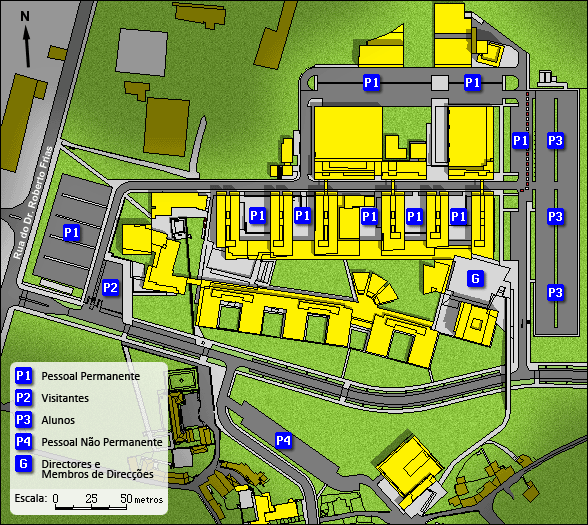
\includegraphics{map.pdf}
    \end{center}
    \caption{Parte do mapa do bloco B}
    \label{fig:map}
  \end{figure}




% section solucao (end)


\section{Conclusões}\label{sec:conclusions}

\lipsum[8]

%----------------------------------------------------------------------------------------
%	REFERENCE LIST
%----------------------------------------------------------------------------------------

%% auto bibliographic list 
\renewcommand{\bibname}{Referências}
% uses bibtex file
%\bibliographystyle{alpha-pt}
%\bibliographystyle{alpha}
\bibliographystyle{unsrt-pt}
%\bibliographystyle{unsrt}
\bibliography{bib/myrefs}

%----------------------------------------------------------------------------------------

\end{document}


